\section{Auswertung}
\label{sec:Auswertung}

Die Graphen werden sowohl mit Matplotlib \cite{matplotlib} als auch NumPy \cite{numpy} erstellt. Die Fehlerrechnung wird mithilfe von Uncertainties \cite{uncertainties} durchgeführt.

\subsection{Die Kennlinien der Diode bei unterschiedlichen Heizspannungen}

In den Abbildungen \ref{fig:Kennlinien} und \ref{fig:Kennlinien2} sind die Kennlinien der Diode bei Heizströmen von $I_.H=\SI{2,1}{\ampere}$ bis $I_.H=\SI{2,5}{\ampere}$ aufgetragen. Die zugehörigen Messwerte befinden sich in den Tabellen \ref{tab:1} und \ref{tab:2}.

\begin{table}
\centering
\caption{Die gemessenen Stromstärken in Abhängigkeit der Beschleunigungsspannung bei Heizströmen von $I_.H=\SI{2,1}{\ampere}$ bis $I_.H=\SI{2,3}{\ampere}$.}
%\label{tab:tab21}
	\sisetup{table-format=1.2}
	\begin{tabular}{S[table-format=3.0]S[table-format=3.0]}
		\toprule
		{$U_\text{B}/\si{\volt}$} & {$I_\text{2,1}/\si{\micro\ampere}$} \\
		\midrule
		  5 &  16 \\
		 10 &  45 \\
		 15 &  75 \\
		 20 & 107 \\
		 25 & 133 \\
		 30 & 153 \\
		 35 & 166 \\
		 40 & 171 \\
		 45 & 181 \\
		 50 & 188 \\
		 55 & 192 \\
		 60 & 198 \\
		 65 & 201 \\
		 70 & 205 \\
		 75 & 210 \\
		 80 & 215 \\
		 85 & 218 \\
		 90 & 220 \\
		 95 & 221 \\
		100 & 222 \\
		105 &   \\
		110 &   \\
		115 &   \\
		120 &   \\
		125 &   \\
		130 &   \\
		135 &   \\
		140 &   \\
		145 &   \\
		150 &   \\
		\bottomrule
	\end{tabular}

%\label{tab:tab22}
	\sisetup{table-format=1.2}
	\begin{tabular}{S[table-format=3.0]S[table-format=3.0]}
		\toprule
		{$U_\text{B}/\si{\volt}$} & {$I_\text{2,2}/\si{\micro\ampere}$} \\
		\midrule
		  5 &   2 \\
		 10 &  54 \\
		 15 &  94 \\
		 20 & 137 \\
		 25 & 185 \\
		 30 & 223 \\
		 35 & 250 \\
		 40 & 262 \\
		 45 & 295 \\
		 50 & 327 \\
		 55 & 358 \\
		 60 & 398 \\
		 65 & 428 \\
		 70 & 449 \\
		 75 & 468 \\
		 80 & 483 \\
		 85 & 497 \\
		 90 & 509 \\
		 95 & 519 \\
		100 & 526 \\
		105 & 533 \\
		110 & 538 \\
		115 & 542 \\
		120 & 546 \\
		125 & 555 \\
		130 & 560 \\
		135 & 563 \\
		\bottomrule
	\end{tabular}

\label{tab:tab21-3}
	\sisetup{table-format=1.2}
	\begin{tabular}{S[table-format=3.0]S[table-format=3.0]S[table-format=3.0]S[table-format=3.0]}
		\toprule
		{$U_\text{B}/\si{\volt}$} & {$I_\text{2,1}/\si{\micro\ampere}$} & {$I_\text{2,2}/\si{\micro\ampere}$} & {$I_\text{2,3}/\si{\micro\ampere}$} \\
		\midrule
		  5 &  16 &   2 &  30 \\
		 10 &  45 &  54 &  70 \\
		 15 &  75 &  94 & 113 \\
		 20 & 107 & 137 & 162 \\
		 25 & 133 & 185 & 196 \\
		 30 & 153 & 223 & 227 \\
		 35 & 166 & 250 & 271 \\
		 40 & 171 & 262 & 318 \\
		 45 & 181 & 295 & 360 \\
		 50 & 188 & 327 & 404 \\
		 55 & 192 & 358 & 453 \\
		 60 & 198 & 398 & 514 \\
		 65 & 201 & 428 & 563 \\
		 70 & 205 & 449 & 609 \\
		 75 & 210 & 468 & 649 \\
		 80 & 215 & 483 & 684 \\
		 85 & 218 & 497 & 718 \\
		 90 & 220 & 509 & 757 \\
		 95 & 221 & 519 & 788 \\
		100 & 222 & 526 & 816 \\
		105 &  NUL  & 533 &  NUL  \\
		110 &  NUL  & 538 & 875 \\
		115 &  NUL  & 542 &  NUL  \\
		120 &  NUL  & 546 & 945 \\
		125 &  NUL  & 555 &  NUL  \\
		130 &  NUL  & 560 & 1003 \\
		135 &  NUL  & 563 &  NUL  \\
		140 &  NUL  &  NUL  & 1057 \\
		145 &  NUL  &  NUL  &  NUL  \\
		150 &  NUL  &  NUL  & 1111 \\
		\bottomrule
	\end{tabular}

\label{tab:1}
\end{table}

\begin{table}
\centering
\caption{Die gemessenen Stromstärken in Abhängigkeit der Beschleunigungsspannung bei Heizströmen von $I_.H=\SI{2,4}{\ampere}$ und $I_.H=\SI{2,5}{\ampere}$.}
%\label{tab:tab24}
	\sisetup{table-format=1.2}
	\begin{tabular}{S[table-format=3.0]S[table-format=4.0]}
		\toprule
		{$U_\text{B}/\si{\volt}$} & {$I_\text{2,4}/\si{\micro\ampere}$} \\
		\midrule
		 10 &   70 \\
		 20 &  171 \\
		 30 &  276 \\
		 40 &  330 \\
		 50 &  430 \\
		 60 &  560 \\
		 70 &  660 \\
		 80 &  774 \\
		 90 &  868 \\
		100 &  945 \\
		110 & 1032 \\
		120 & 1125 \\
		130 & 1205 \\
		140 & 1208 \\
		150 & 1402 \\
		160 & 1492 \\
		170 & 1583 \\
		180 & 1669 \\
		190 & 1753 \\
		200 & 1835 \\
		210 &  NUL  \\
		220 &  NUL  \\
		230 &  NUL  \\
		240 &  NUL  \\
		250 &  NUL  \\
		\bottomrule
	\end{tabular}

\label{tab:tab24-5}
	\sisetup{table-format=1.2}
	\begin{tabular}{S[table-format=3.0]S[table-format=4.0]S[table-format=4.0]}
		\toprule
		{$U_\text{B}/\si{\volt}$} & {$I_\text{2,4}/\si{\micro\ampere}$} & {$I_\text{2,5}/\si{\micro\ampere}$} \\
		\midrule
		 10 &   70 &   67 \\
		 20 &  171 &  174 \\
		 30 &  276 &  286 \\
		 40 &  330 &  342 \\
		 50 &  430 &  444 \\
		 60 &  560 &  574 \\
		 70 &  660 &  695 \\
		 80 &  774 &  815 \\
		 90 &  868 &  942 \\
		100 &  945 & 1031 \\
		110 & 1032 & 1137 \\
		120 & 1125 & 1250 \\
		130 & 1205 & 1337 \\
		140 & 1208 & 1461 \\
		150 & 1402 & 1596 \\
		160 & 1492 & 1709 \\
		170 & 1583 & 1835 \\
		180 & 1669 & 1971 \\
		190 & 1753 & 2110 \\
		200 & 1835 & 2240 \\
		210 &  NUL  & 2390 \\
		220 &  NUL  & 2520 \\
		230 &  NUL  & 2600 \\
		240 &  NUL  & 2810 \\
		250 &  NUL  & 2950 \\
		\bottomrule
	\end{tabular}

\label{tab:2}
\end{table}

\begin{figure}
\centering
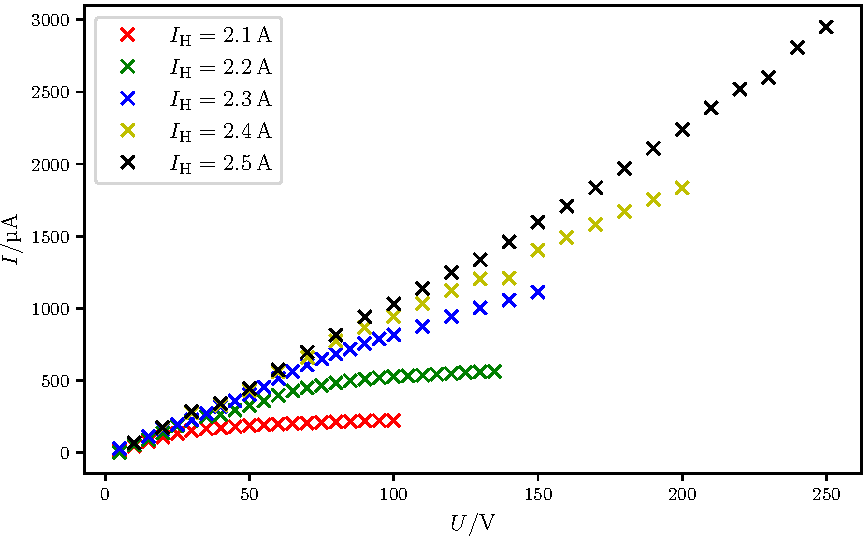
\includegraphics[width=\linewidth-70pt,height=\textheight-70pt,keepaspectratio]{content/images/IH_21-5.pdf}
\caption{Die Kennlinien der Diode bei Heizströmen von $I_.H=\SI{2,1}{\ampere}$ bis $I_.H=\SI{2,5}{\ampere}$.}
\label{fig:Kennlinien}
\end{figure}

\begin{figure}
\centering
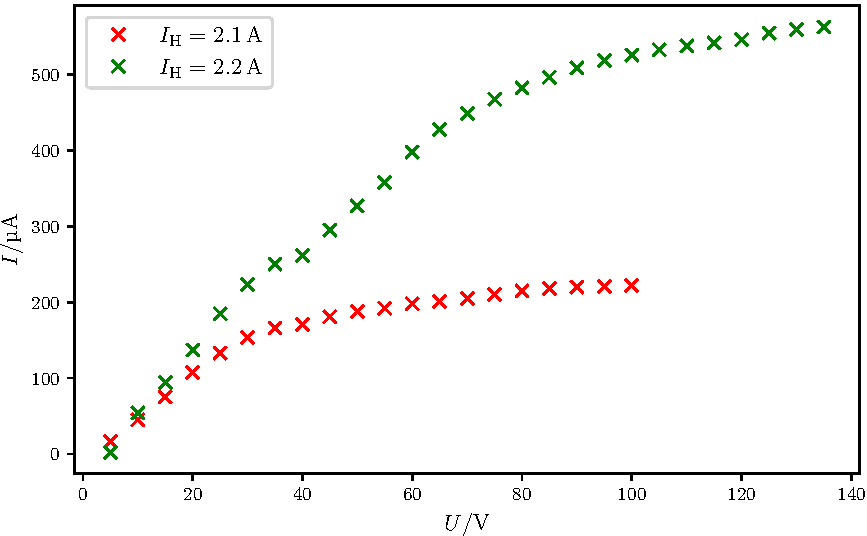
\includegraphics[width=\linewidth-70pt,height=\textheight-70pt,keepaspectratio]{content/images/IH_21-2.pdf}
\caption{Die Kennlinien der Diode bei Heizströmen von $I_.H=\SI{2,1}{\ampere}$ und $I_.H=\SI{2,2}{\ampere}$.}
\label{fig:Kennlinien2}
\end{figure}

\subsection{Bestimmung des Exponenten der Strom-Spannungs-Beziehung im Raumladungsgebiet}
\label{subsec:Exponent}

Bei dem Heizstrom $I_.H=\SI{2,5}{\ampere}$ kann die gesamte Kennlinie als Raumladungsgebiet betrachtet werden.
Mithilfe von Formel \eqref{eq:langmuir} und einer linearen Ausgleichsrechnung der Form $\log(I)=a\log(U)+b$ ergibt sich mit den Werten aus Tabelle \ref{tab:2} für den Exponenten a in der Strom-Spannungs-Beziehung:
\begin{align*}
a &= 1,14\pm0,01\text{,}\\
b &= \SI{-12.14(4)}{\log\left(\ampere\per\volt\tothe{a}\right)}\text{.}
\end{align*}

\begin{figure}
\centering
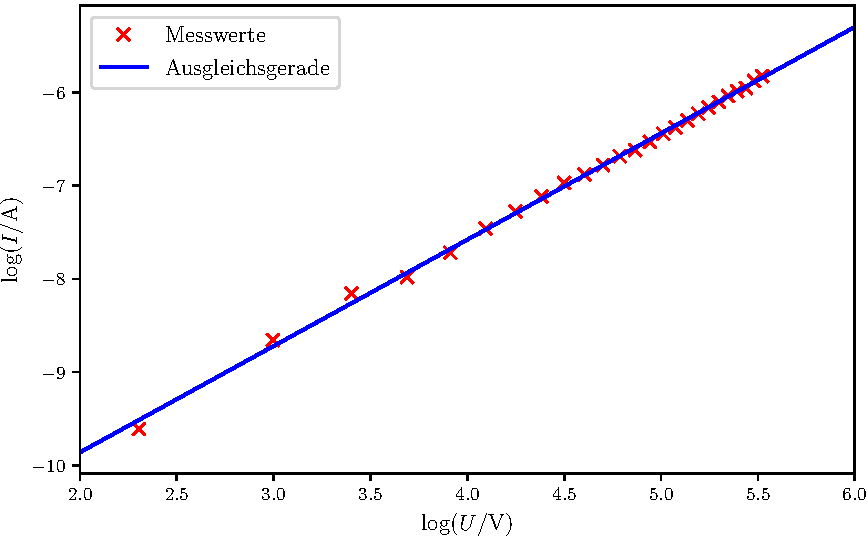
\includegraphics[width=\linewidth-70pt,height=\textheight-70pt,keepaspectratio]{content/images/IH_25_log.pdf}
\caption{Die Kennlinie der Diode bei einem Heizstrom von $I_.H=\SI{2,5}{\ampere}$ in logarithmischer Darstellung im Raumladungsgebiet.}
\label{fig:Kennlinie25_log}
\end{figure}

\subsection{Bestimmung der Kathodentemperatur über den Anlaufstrom}
\label{subsec:Temperatur}

Mithilfe der Werte aus Tabelle \ref{tab:Anlaufstrom} wird eine lineare Ausgleichsrechnung der Form $\log(I)=\alpha U+\beta$ durchgeführt:
\begin{align*}
\alpha &= \SI{4,3(2)}{\per\volt}\text{,}\\
\beta  &= \SI{-16.44(9)}{\log(\ampere)}\text{.}
\end{align*}
Dabei wird bei der Spannung der Innenwiderstand des Amperemeters von $R_.i=\SI{1}{\mega\ohm}$ berücksichtigt. Mit Formel \eqref{eq:Anlauf} ergibt sich:
\[
T = \frac{e_0}{k_.B\alpha} = \SI{2.7(1)e3}{\kelvin}\text{.}
\]
Die Werte aus der Tabelle sind in Abbildung \ref{fig:Anlaufstrom} graphisch dargestellt.

\begin{table}
\centering
\caption{Die gemessenen Stromstärken in Abhängigkeit der Beschleunigungsspannung bei einem Heizstrom von $I_.H=\SI{2,5}{\ampere}$ im Bereich des Anlaufstromes.}
\label{tab:tabAnlaufstrom}
	\sisetup{table-format=1.2}
	\begin{tabular}{S[table-format=0.2]S[table-format=2.1]}
		\toprule
		{$U_\text{B}/\si{\volt}$} & {$I_\text{Anlauf}/\si{\nano\ampere}$} \\
		\midrule
		0.09 & 85.0 \\
		-0.05 & 55.0 \\
		-0.16 & 36.0 \\
		-0.28 & 23.0 \\
		-0.38 & 16.2 \\
		-0.49 & 10.0 \\
		-0.59 & 7.0 \\
		-0.70 & 4.0 \\
		-0.80 & 2.4 \\
		-0.90 & 1.3 \\
		-0.92 & 1.0 \\
		\bottomrule
	\end{tabular}

\label{tab:Anlaufstrom}
\end{table}

\begin{figure}
\centering
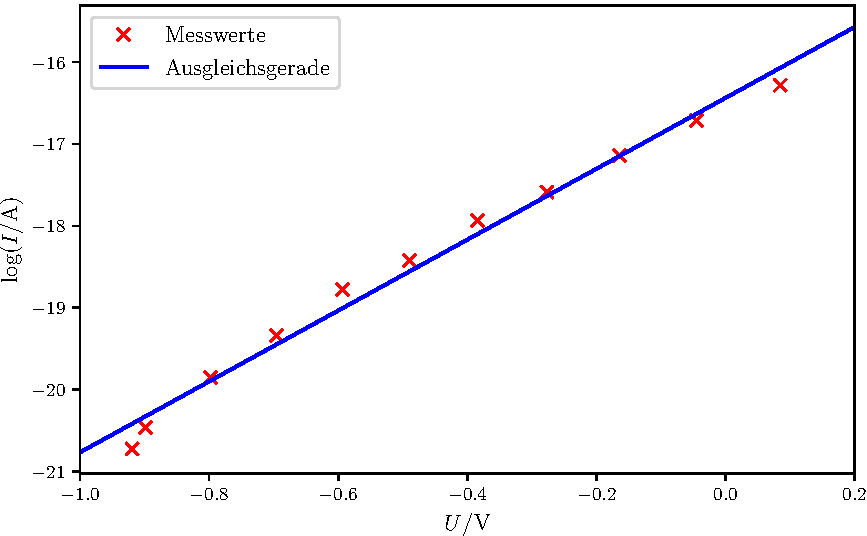
\includegraphics[width=\linewidth-70pt,height=\textheight-70pt,keepaspectratio]{content/images/Anlaufstrom.pdf}
\caption{Die Kennlinie der Diode bei einem Heizstrom von $I_.H=\SI{2,5}{\ampere}$ in halb-logarithmischer Darstellung im Bereich des Anlaufstroms.}
\label{fig:Anlaufstrom}
\end{figure}

\subsection{Bestimmung des Sättigungsstromes, der Kathodentemperatur und der Austrittsarbeit der Diode}

Der Sättigungsstrom $I_.S$ in Tabelle \ref{tab:STA} wird mithilfe der Abbildungen \ref{fig:Kennlinien} und \ref{fig:Kennlinien2} abgeschätzt.
Die Leistung $W_.H$ errechnet sich durch $W_.H = I_.H U_.H$.
Die Temperatur $T_.S$ berechnet sich nach Formel \eqref{eq:T}. Dabei wird ein Leistungsverlust durch die Wärmeleitung von $N_.{WL}=\SI{1}{\watt}$ angenommen. Die emittierende Kathodenoberfläche beträgt $A = \SI{0.32}{\centi\metre\squared}$. $\sigma=\SI{5.7e-12}{\watt\per\centi\per\metre\squared\per\kelvin\tothe{4}}$ ist die Stefan-Bolzmannsche Strahlungskonstante und $\eta=0,28$ der Emissionsgrad der Oberfläche \cite{V504}.
Die Austrittsarbeit $\phi$ in der Tabelle berechnet sich nach Umformen von Formel \eqref{eq:IS} durch:
\[
\phi = -\log\left(\frac{I_.Sh^3}{4\pi e_0m_0Ak_.B^2T^2}\right)\frac{k_.BT}{e_0}\text{.}
\]
Für die mittlere Austrittsarbeit $\bar{\phi}$ ergibt sich demnach mit der Formel für den Mittelwert
\[
\phi_\mu = \frac{1}{N}\sum_i\phi_i
\]
und die Standartabweichung
\[
\sigma_.{\phi}=\sqrt{\frac{1}{N^2-N}\sum_i \left(\phi_i-\phi_\mu\right)^2}
\]
mit den Werten aus der Tabelle ein Wert von
\[
\bar{\phi} = \SI{4.799(8)}{\electronvolt}\text{.}
\]

\begin{table}
\centering
\caption{Die Heizspannung $I_.H$,die Heizleistung $W_.H$ und die geschätzten Werte für den Sättigungsstrom $I_.S$, sowie die berechneten Werte für die Kathodentemperatur $T_.S$ und die Austrittsarbeit $\phi$.}
\label{tab:tabSTA}
	\sisetup{table-format=1.2}
	\begin{tabular}{S[table-format=1.1]S[table-format=1.2]S[table-format=2.1]S[table-format=4.0]S[table-format=3.0]S[table-format=1.2]}
		\toprule
		{$I_\text{H}/\si{\ampere}$} & {$U_\text{H}/\si{\volt}$} & {$W_\text{H}/\si{\watt}$} & {$I_\text{S}/\si{\micro\ampere}$} & {$T_\text{S}/\si{\kelvin}$} & {$\phi/\si{\electronvolt}$} \\
		\midrule
		2.1 & 4.75 & 10.0 &  230 & 2047 & 4.81 \\
		2.2 & 5.00 & 11.0 &  600 & 2104 & 4.78 \\
		2.3 & 5.50 & 12.6 & 1500 & 2185 & 4.81 \\
		2.4 & 5.95 & 14.3 & 3500 & 2258 & 4.82 \\
		2.5 & 6.00 & 15.0 & 6000 & 2288 & 4.78 \\
		\bottomrule
	\end{tabular}

\label{tab:STA}
\end{table}